\documentclass[a4paper,10pt]{article}

%Packages
\usepackage{txfonts}
\usepackage{titlesec}
\usepackage[utf8]{inputenc}
\usepackage[T1]{fontenc}
\usepackage{geometry}
\usepackage{graphicx}
\usepackage{multicol}
\usepackage{fancyhdr}
\usepackage{hyperref}
\usepackage{float}
\usepackage{setspace}
\usepackage{caption}
\usepackage{booktabs}

% PAGE LAYOUT
\geometry{a4paper, top=18mm, bottom=18mm, textwidth=185mm}
\setlength{\columnsep}{6mm}
\setlength{\parindent}{0pt}

\titleformat{\section}
{\normalfont\bfseries}
	{\thesection.}{0.5em}{}
\titleformat{\subsection}
	{\normalfont\itshape}
	{\thesubsection.}{0.5em}{}

\pagestyle{fancy}
\renewcommand{\footrulewidth}{0pt}
\fancyhf{}
\rhead{
\includegraphics[scale=0.4]{Images/hepia_simple.png}}
\rfoot{\textit{\today}}
\cfoot{\thepage}

\captionsetup{
  font=footnotesize,
  labelsep=colon
}

\begin{document}

\begin{multicols*}{2}
[
\begin{center}
\vspace*{0mm}
{\large
AI in Healthcare – Medical Image Analysis \\
\vspace{3mm}
Polyp Characterization and Semantic Segmentation
}\\
\vspace{8mm}
Guilhem Rozier Vilardell\footnote{\textit{\href{mailto:guroz26@student.sdu.dk}{guroz26@student.sdu.dk}}}
\\
\vspace{3mm}
\footnotesize{
\textit{AI in Healthcare Summer Camp – Medical Image Analysis}
}\\
\vspace{9mm}
\end{center}
\rule{\linewidth}{0.4pt}
\onehalfspacing
\textbf{Abstract}\\
This report presents two medical image analysis tasks: polyp characterization (binary classification) using DenseNet121 and semantic segmentation of neuronal membranes using Attention U-Net. For Task 1, we implemented DenseNet121 pretrained on ImageNet with a binary classification head for CCE polyp characterization. The model achieved strong performance: 96.49\% accuracy, 94.19\% sensitivity, 98.17\% specificity, F1 score of 0.958, and AUC of 0.990. Early stopping with patience 5 prevented overfitting. For Task 2, we implemented Attention U-Net with DiceBCE loss for membrane segmentation. The model achieved a Jaccard index of 0.717, F1 score of 0.835, recall of 0.878, precision of 0.797, and accuracy of 0.921 on the training set, with a pixel-level AUC of 0.970. Both models demonstrate the effectiveness of deep learning for medical image analysis tasks, with DenseNet121 particularly well-suited for small datasets due to its parameter efficiency and Attention U-Net's attention gates helping segmentation quality on a very small (24-image) training set.\\
\noindent\textit{Keywords:} medical image analysis, polyp characterization, semantic segmentation, DenseNet121, Attention U-Net, DiceBCE loss\\
\rule{\linewidth}{0.4pt}
]
\singlespacing

\tableofcontents

\setlength{\parskip}{1pt}
\columnbreak

\section{Introduction}
Medical image analysis has become a crucial application of deep learning, particularly in oncology and pathology. This report covers two fundamental tasks: (i) binary classification for polyp characterization in Capsule Colon Endoscopy (CCE) images, and (ii) semantic segmentation of neuronal membranes from electron microscopy images.

Colorectal cancer is the third most common cancer and second leading cause of cancer-related mortality. Early detection through polyp identification can significantly reduce mortality rates. CCE offers a less invasive alternative to traditional colonoscopy but presents challenges: lower image resolution, missing regions of interest, and polyp variability. Similarly, neuronal membrane segmentation from electron microscopy images is essential for connectomics research, where UNet-family architectures (here, Attention U-Net) have become a standard approach.

\section{Polyp Characterization}

\subsection{Model Description: DenseNet121}
DenseNet introduces dense connectivity where each layer receives inputs from all preceding layers within a dense block. Instead of adding feature maps like ResNet's skip connections, DenseNet concatenates them: \(x_\ell = H_\ell([x_0, x_1, ..., x_{\ell-1}])\). This concatenation is the key structural difference.

The DenseNet121 architecture consists of 4 dense blocks (with 6, 12, 24, and 16 layers respectively). Each block uses a bottleneck design: \(1 \times 1\) convolution followed by \(3 \times 3\) convolution with preactivation. Transition layers (1x1 conv + 2x2 average pooling) between blocks compress channel count and reduce spatial resolution. The growth rate \(k=32\) determines how many new feature maps each layer adds.

DenseNet is particularly suitable for this task for two reasons: 
\begin{itemize}
	\item Feature reuse reduces parameters compared to ResNet or VGG of similar depth, which is crucial given the limited CCE dataset size.
	\item It is a well-established baseline in medical imaging (e.g., CheXNet for chest X-rays) due to its parameter efficiency on limited labeled data. The trade-off is higher memory consumption during training since activations must be kept for the entire dense block.
\end{itemize}

\subsection{Data Preparation}
The CCE dataset consists of RGB images of resolution \(512 \times 512\), resized to \(224 \times 224\) for compatibility with ImageNet-pretrained models. Binary classification labels: Non-neoplasia (class 0) and Neoplasia (class 1). The dataset was split into training (1667 images), validation (562 images), and test (569 images) sets using provided text files.

Data augmentation on the training set included random horizontal flips and rotations (\(\pm10^\circ\)), with normalization using mean and standard deviation of 0.5 across all channels.

\subsection{Implementation Details}
We used DenseNet121 pretrained on ImageNet via PyTorch's torchvision library. The classifier head was replaced with a single neuron for binary classification. Loss function: Binary Cross-Entropy with Logits Loss (BCEWithLogitsLoss). Optimizer: Adam with learning rate \(10^{-4}\) and betas \((0.9, 0.999)\). Early stopping with patience 5: training stopped after 10 epochs when validation loss stopped improving for 5 consecutive epochs (best checkpoint, from epoch 5, restored). Batch size: 32.

\subsection{Results}
Figure~\ref{fig:densenet_curves} shows training and validation loss and accuracy over epochs. The model converged quickly: validation accuracy rose from 84.16\% at epoch 1 to 94.48\% by epoch 2, then fluctuated in the 94-97\% range while training accuracy climbed steadily from 76.84\% to 99.40\% by epoch 10, with a growing train/validation gap indicating mild overfitting. Validation loss reached its minimum (0.0961) at epoch 5 and rose thereafter (peaking at 0.1758 at epoch 7 before settling around 0.14); early stopping (patience 5) triggered at epoch 10, restoring the epoch-5 checkpoint.

\begin{figure}[H]
\centering
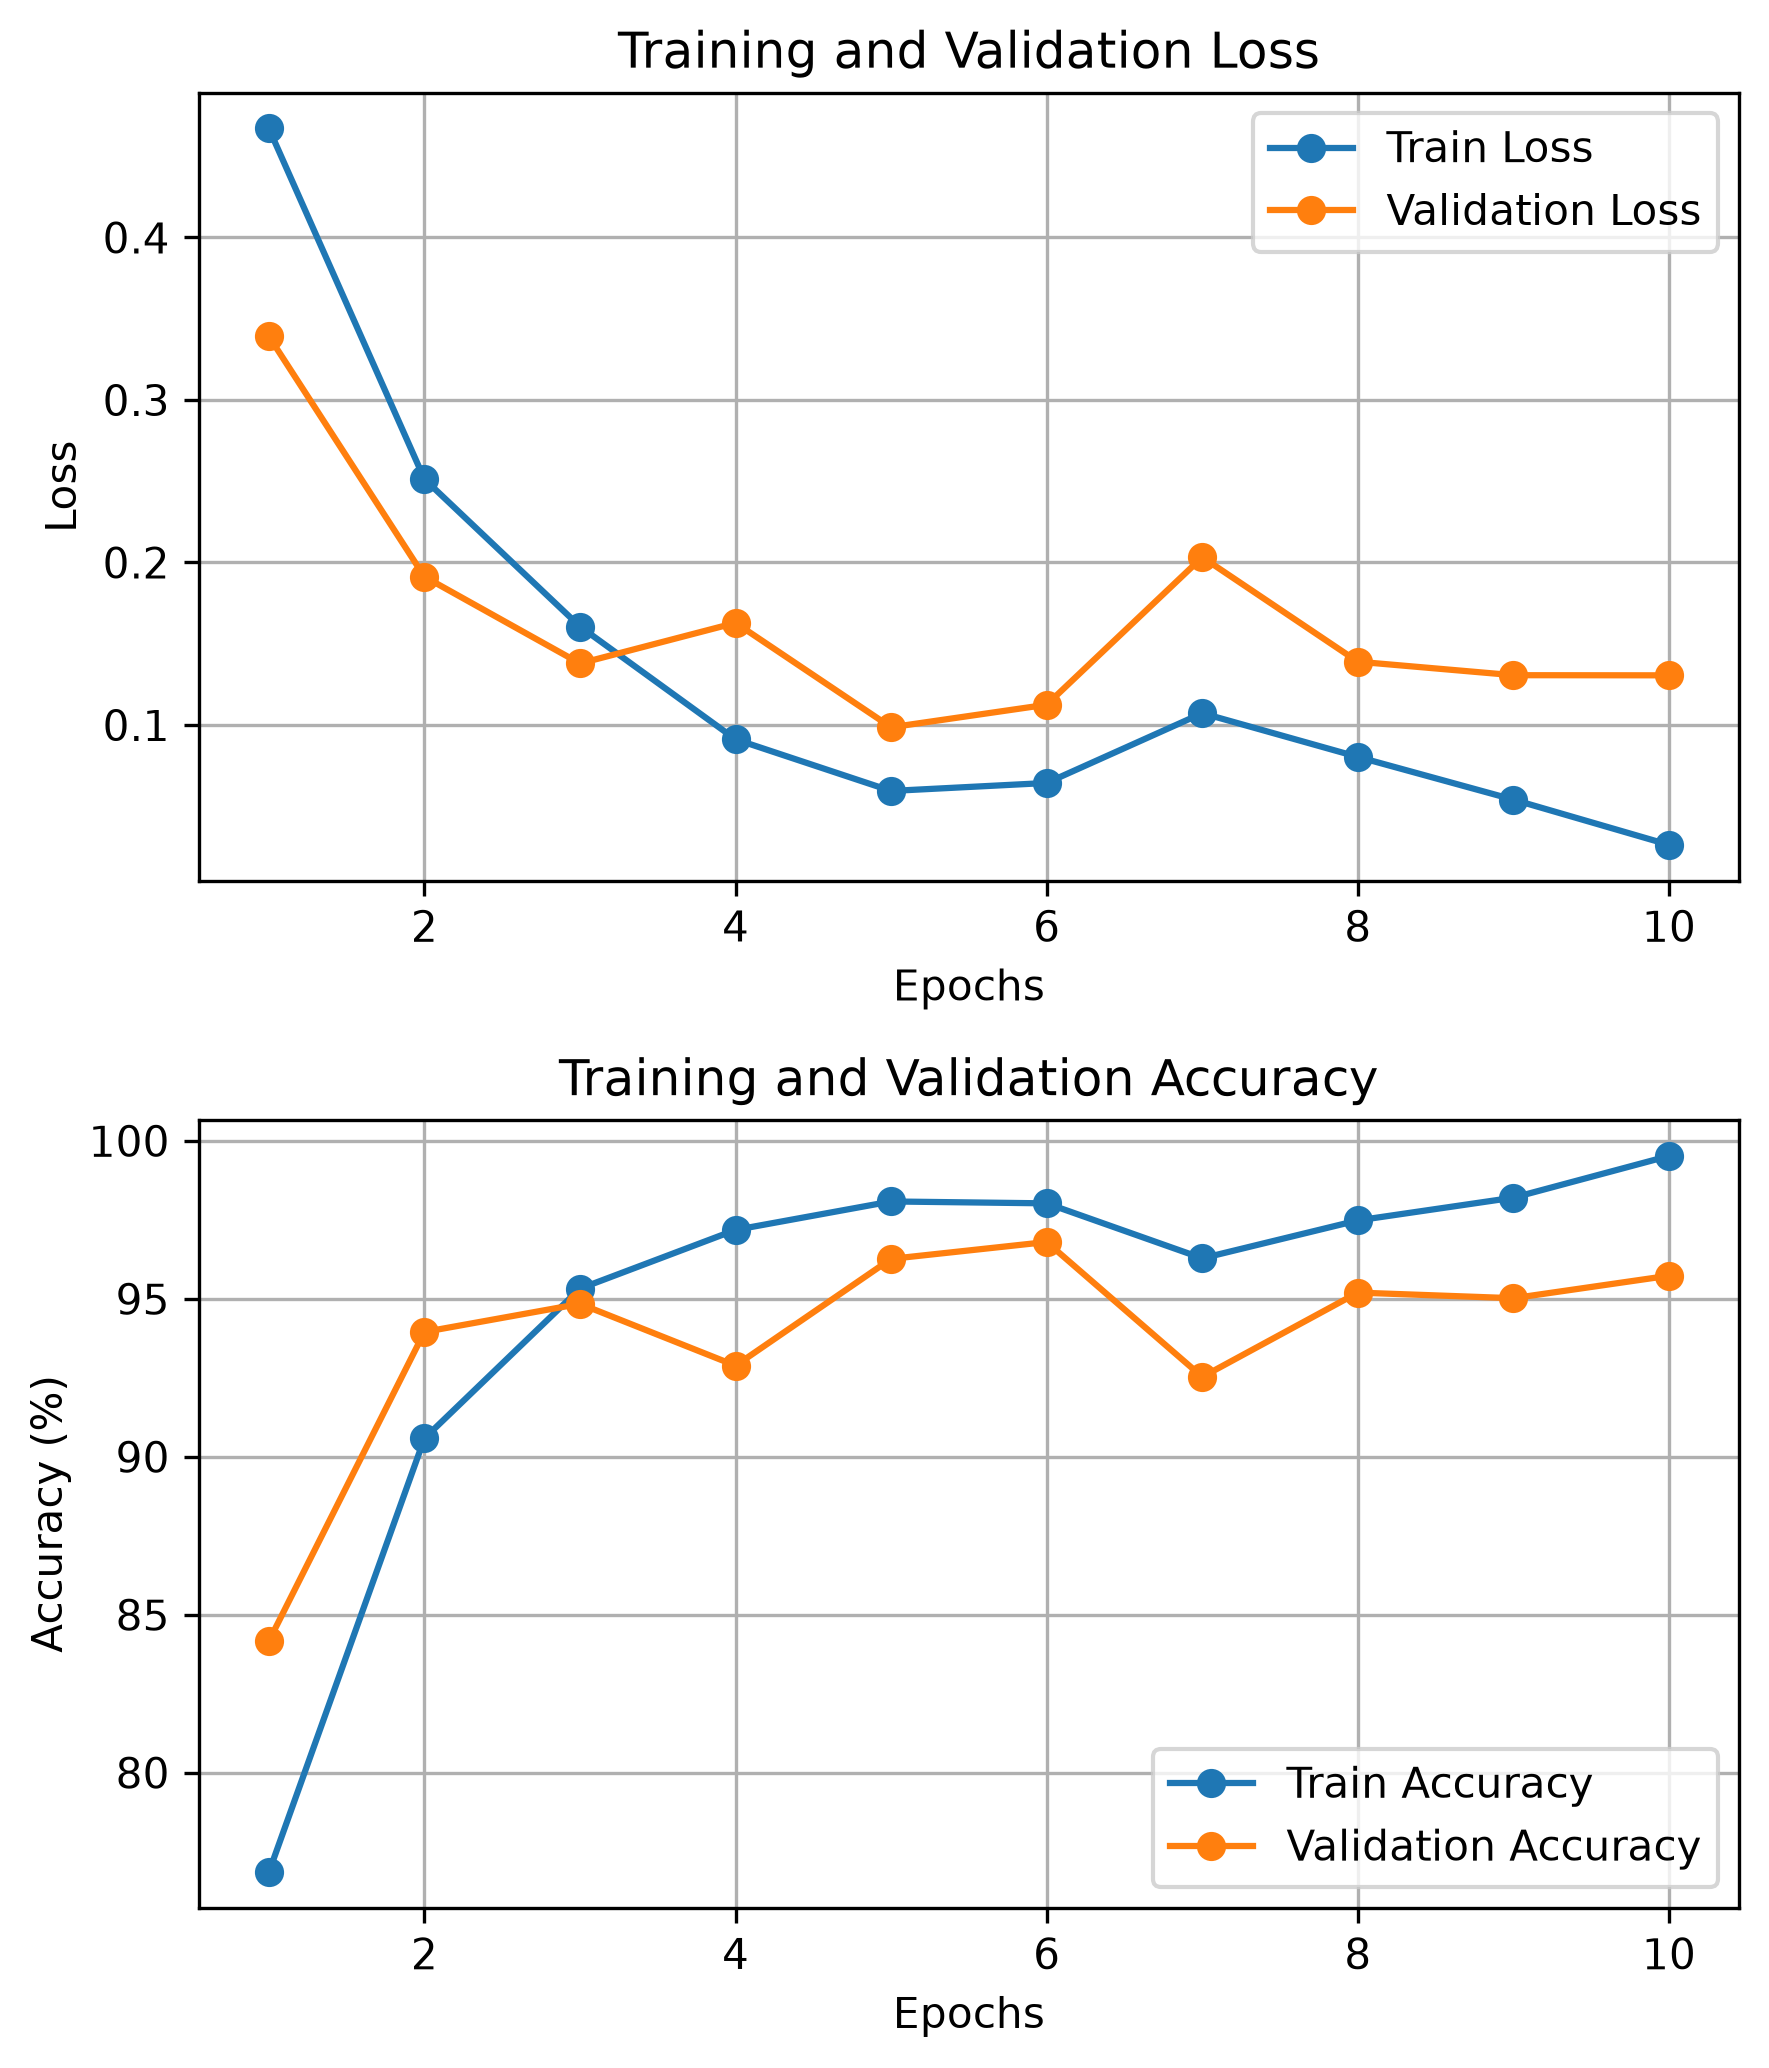
\includegraphics[width=\linewidth]{Images/densenet121_training_curves.png}
\caption{Training and validation curves for DenseNet121.}
\label{fig:densenet_curves}
\end{figure}

Table~\ref{tab:densenet_perf} reports comprehensive performance metrics on the test set (569 images). The model misclassified 20 of 569 images (confusion matrix shown in Figure~\ref{fig:densenet_confusion}): 6 false positives and 14 false negatives.

\begin{table}[H]
\centering
\caption{DenseNet121 test performance.}
\label{tab:densenet_perf}
\begin{tabular}{lr}
\toprule
Metric & Value \\
\midrule
Accuracy (\%) & 96.49 \\
Sensitivity (\%) & 94.19 \\
Specificity (\%) & 98.17 \\
F1 Score & 0.9578 \\
AUC & 0.9930 \\
\bottomrule
\end{tabular}
\end{table}

\begin{figure}[H]
\centering
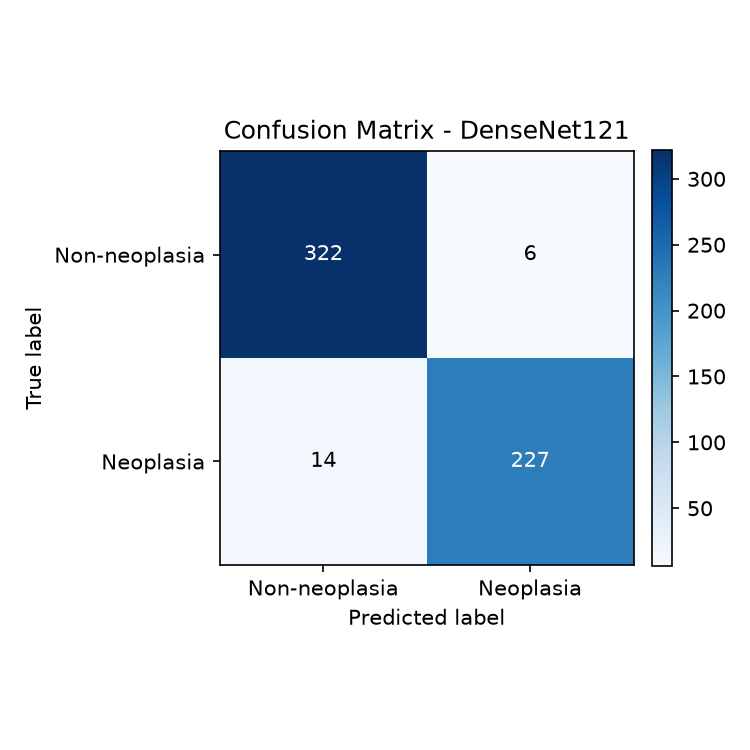
\includegraphics[width=0.8\linewidth]{Images/densenet121_confusion_matrix.png}
\caption{Confusion matrix - DenseNet121.}
\label{fig:densenet_confusion}
\end{figure}

The ROC curve (Figure~\ref{fig:densenet_roc}) gives an AUC of 0.993, not perfect but still excellent discriminative ability; the curve sits close to the top-left corner across nearly the full false-positive-rate range. The Precision-Recall curve (Figure~\ref{fig:densenet_pr}) shows precision holding at essentially 1.0 up to recall $\approx$0.8, then degrading sharply as recall approaches 1.0, meaning the last few positives are only recoverable at a steep precision cost -- consistent with the 20 misclassifications in Table~\ref{tab:densenet_perf}.

\begin{figure}[H]
\centering
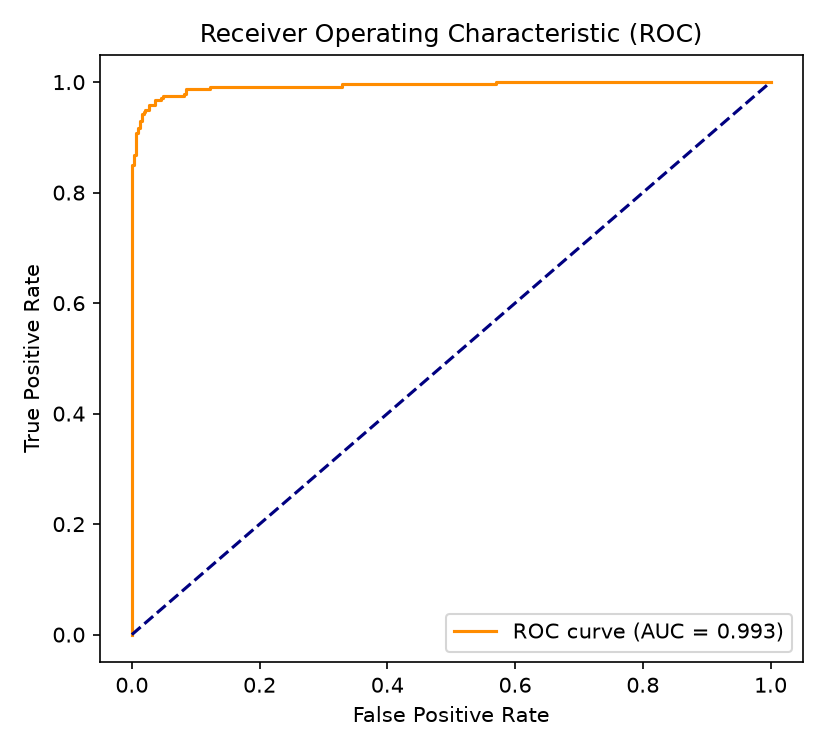
\includegraphics[width=0.8\linewidth]{Images/densenet121_roc.png}
\caption{ROC curve - DenseNet121 (AUC = 0.993).}
\label{fig:densenet_roc}
\end{figure}

\begin{figure}[H]
\centering
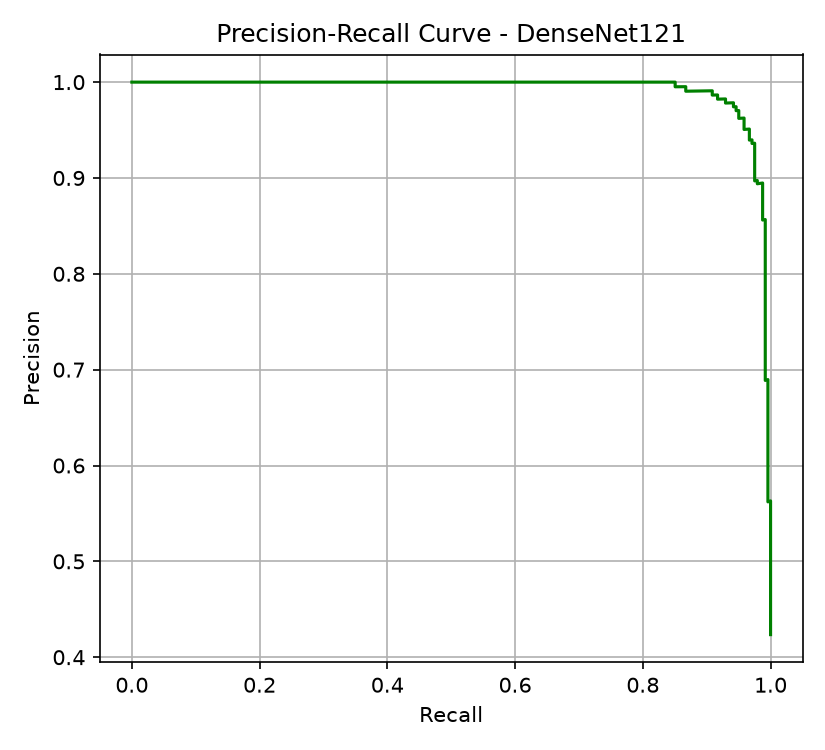
\includegraphics[width=0.8\linewidth]{Images/densenet121_pr_curve.png}
\caption{Precision-Recall curve - DenseNet121.}
\label{fig:densenet_pr}
\end{figure}

Figure~\ref{fig:densenet_gradcam} shows Grad-CAM heatmaps overlaid on test images, highlighting the regions the model focused on when making predictions. The attention is concentrated on polyp regions, validating that the model learns clinically relevant features.

\begin{figure}[H]
\centering
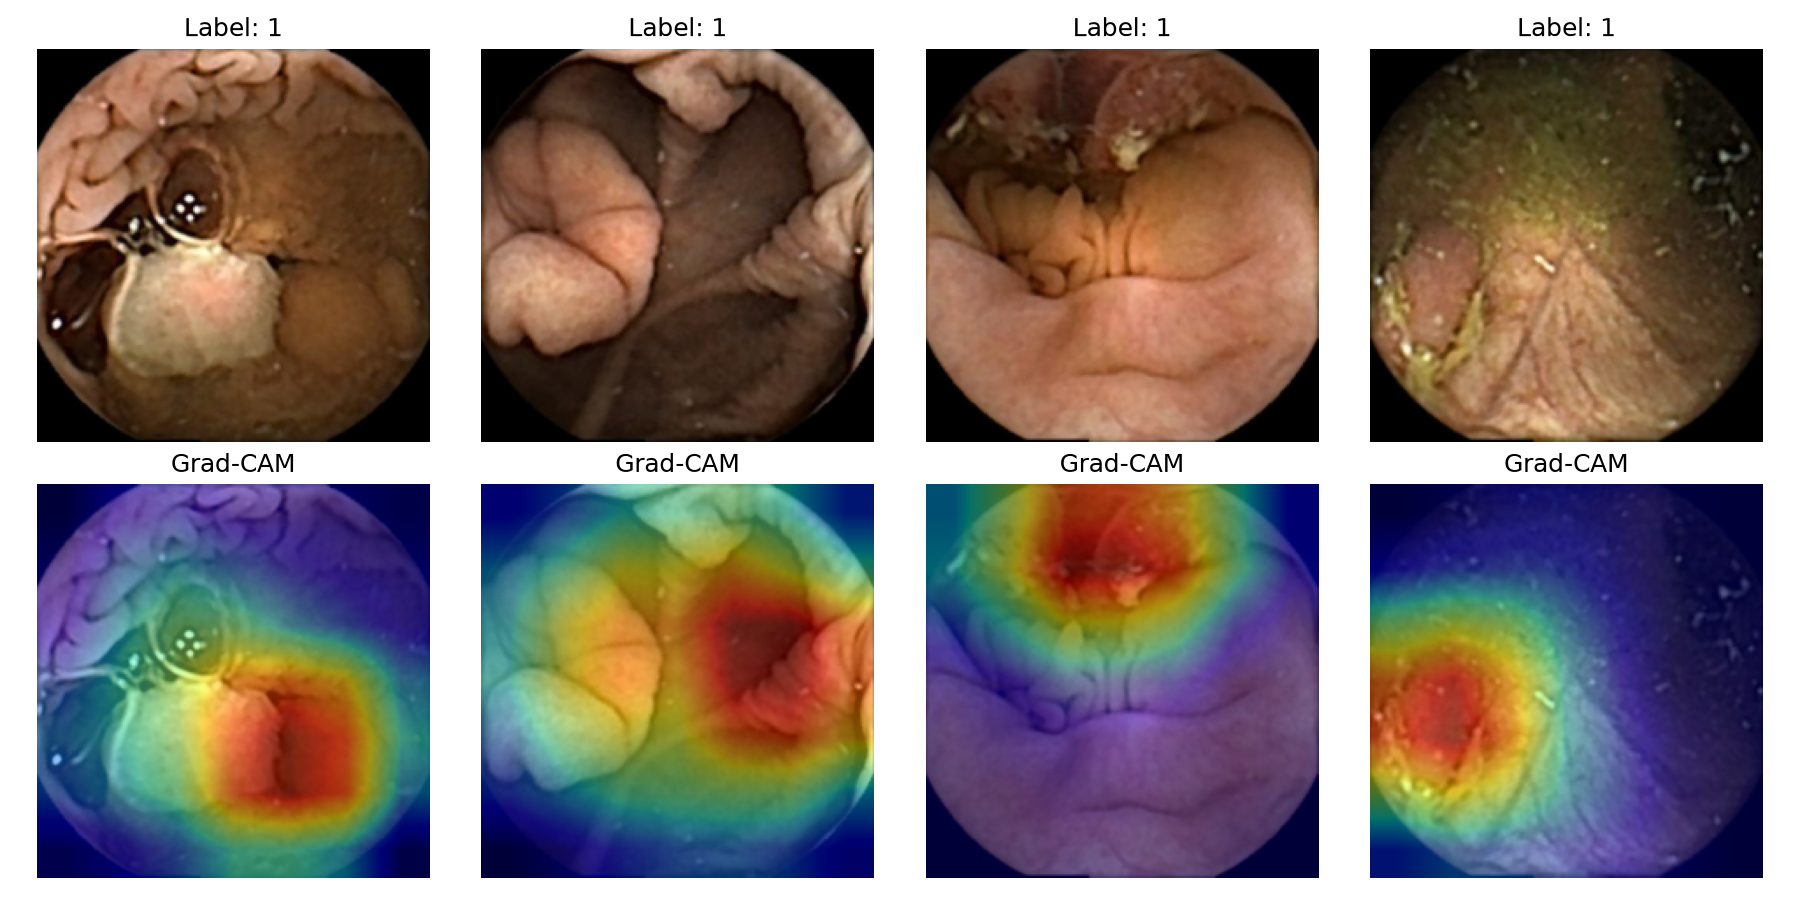
\includegraphics[width=\linewidth]{Images/densenet121_gradcam.png}
\caption{Grad-CAM visualizations on test samples.}
\label{fig:densenet_gradcam}
\end{figure}

Table~\ref{tab:model_comparison} compares our DenseNet121 (pretrained) with a scratch-trained ResNet18 and a pretrained MobileNet from group members.

\begin{table}[H]
\centering
\caption{Model comparison for polyp characterization.}
\label{tab:model_comparison}
\small
\setlength{\tabcolsep}{3.5pt}
\begin{tabular}{l c c c c c c}
\toprule
Model & Type & Acc. & Sens. & Spec. & F1 & AUC \\
\midrule
DenseNet121 & Pretr. & 96.49 & 94.19 & 98.17 & 0.9580 & 0.9930 \\
ResNet18   & Scratch & 94.31 & 95.24 & 93.55 & 0.9375 & 0.9846 \\
MobileNet  & Pretr. & 95.02 & 91.27 & 98.06 & 0.9426 & 0.9895 \\
\bottomrule
\end{tabular}
\end{table}

This comparison highlights three points. 
\begin{itemize}
	\item Both pretrained backbones (DenseNet121, MobileNet) beat the scratch-trained ResNet18 on accuracy, specificity, and AUC, suggesting ImageNet pretraining is the dominant factor on this $\sim$1700-image training set.
	\item DenseNet121 and MobileNet reach similar AUC ($\geq$0.989 both) but trade off differently: DenseNet121's sensitivity (94.19\%) exceeds MobileNet's (91.27\%) at effectively no specificity cost (98.17\% vs 98.06\%), which matters clinically since a missed neoplasia (false negative) is costlier than a false alarm.
	\item ResNet18's specificity (93.55\%) trails both pretrained models by $\sim$4.5 points despite its highest sensitivity (95.24\%) of the three -- it over-predicts the positive class, consistent with a from-scratch model on a training set well below typical data requirements for that regime.
\end{itemize}


\section{Task 2: Semantic Segmentation}

\subsection{Model Description: Attention U-Net}
Attention U-Net keeps UNet's symmetric, full-resolution encoder-decoder with skip connections, but adds an attention gate on every skip connection: before concatenation, each encoder feature map is gated by a signal computed jointly from itself and the corresponding decoder feature map, letting the decoder suppress irrelevant background instead of relying on capacity learned from scratch to do so -- the mechanism the original paper reports helps most on small datasets. GroupNorm replaces BatchNorm throughout (stable statistics at batch size 2). Channel width follows 16 → 32 → 64 → 128 → 256 (base width 16, half of the standard UNet's 64) across 4 downsampling stages plus a bottleneck; each encoder/decoder stage is a double 3x3-conv block (GroupNorm + ReLU), downsampling via 2x2 max pooling and upsampling via 2x2 transposed convolutions. A final 1x1 convolution plus sigmoid produces the per-pixel membrane probability. As in the original UNet exercise setup, inputs are reflection-padded to 572x572 and outputs are center-cropped to 388x388, though internally the convolutions use padding=1, so the size reduction here comes purely from the explicit crop rather than from unpadded convolutions.\\


Attention U-Net is well suited for our dataset because the attention gates let the model focus its limited capacity on membrane boundaries without needing more labeled data to learn that focus implicitly, and full-resolution skip connections preserve the fine spatial detail membrane segmentation depends on.

\subsection{Data Preparation}
Our dataset consists of 30 labeled training images (512 × 512 pixels) and 30 unlabeled test images. Binary labels: membrane pixels (foreground) and background. Ground truth convention: membrane pixels are dark (value < 128), converted to 1, background to 0.

Input images were padded to 572 × 572 using reflection padding, then center-cropped to 388 × 388 after the forward pass. Training split: 24 slices for training, 6 for validation (early stopping only). Augmentation included random horizontal and vertical flips. Per instructor feedback, the full 30-slice labeled set (not the 6-slice validation split) was used for final performance reporting, since the unlabeled test set has no ground truth to evaluate against; the 6-slice validation split is used only for early-stopping model selection during training.

\subsection{Implementation Details}
Loss function: DiceBCE Loss, combining Binary Cross-Entropy and Dice Losswith \(p_i\) the predicted probability, \(g_i\) the ground truth label, and \(\epsilon = 10^{-6}\) for numerical stability.\\

Optimizer: Adam with learning rate \(10^{-4}\). Early stopping with patience 5: training stopped after 55 epochs when validation loss stopped improving for 5 consecutive epochs (best checkpoint, from epoch 50, restored). Batch size: 2 (to use limited GPU memory for 572 × 572 inputs). Number of epochs: 100 (upper bound, early stopped at 55).

\subsection{Results}
Figure~\ref{fig:unet_curves} shows training and validation loss, and validation IoU over epochs. The DiceBCE loss decreased smoothly and almost equally from $\approx$1.27 (train) / $\approx$1.21 (val) at epoch 1 to 0.5665 (train) / 0.6235 (val) at epoch 55, with train and validation loss tracking closely until roughly epoch 30-35, after which validation loss plateaus around 0.62-0.65 while training loss keeps falling -- a mild overfitting gap consistent with only 24 training slices. Validation IoU rose steeply over the first $\approx$10 epochs (0.39 to 0.62), then continued climbing more gradually with epoch-to-epoch noise, reaching its best value ($\approx$0.679, val loss 0.6163) at epoch 50; early stopping (patience 5) triggered at epoch 55, restoring the epoch-50 checkpoint.

\begin{figure}[H]
\centering
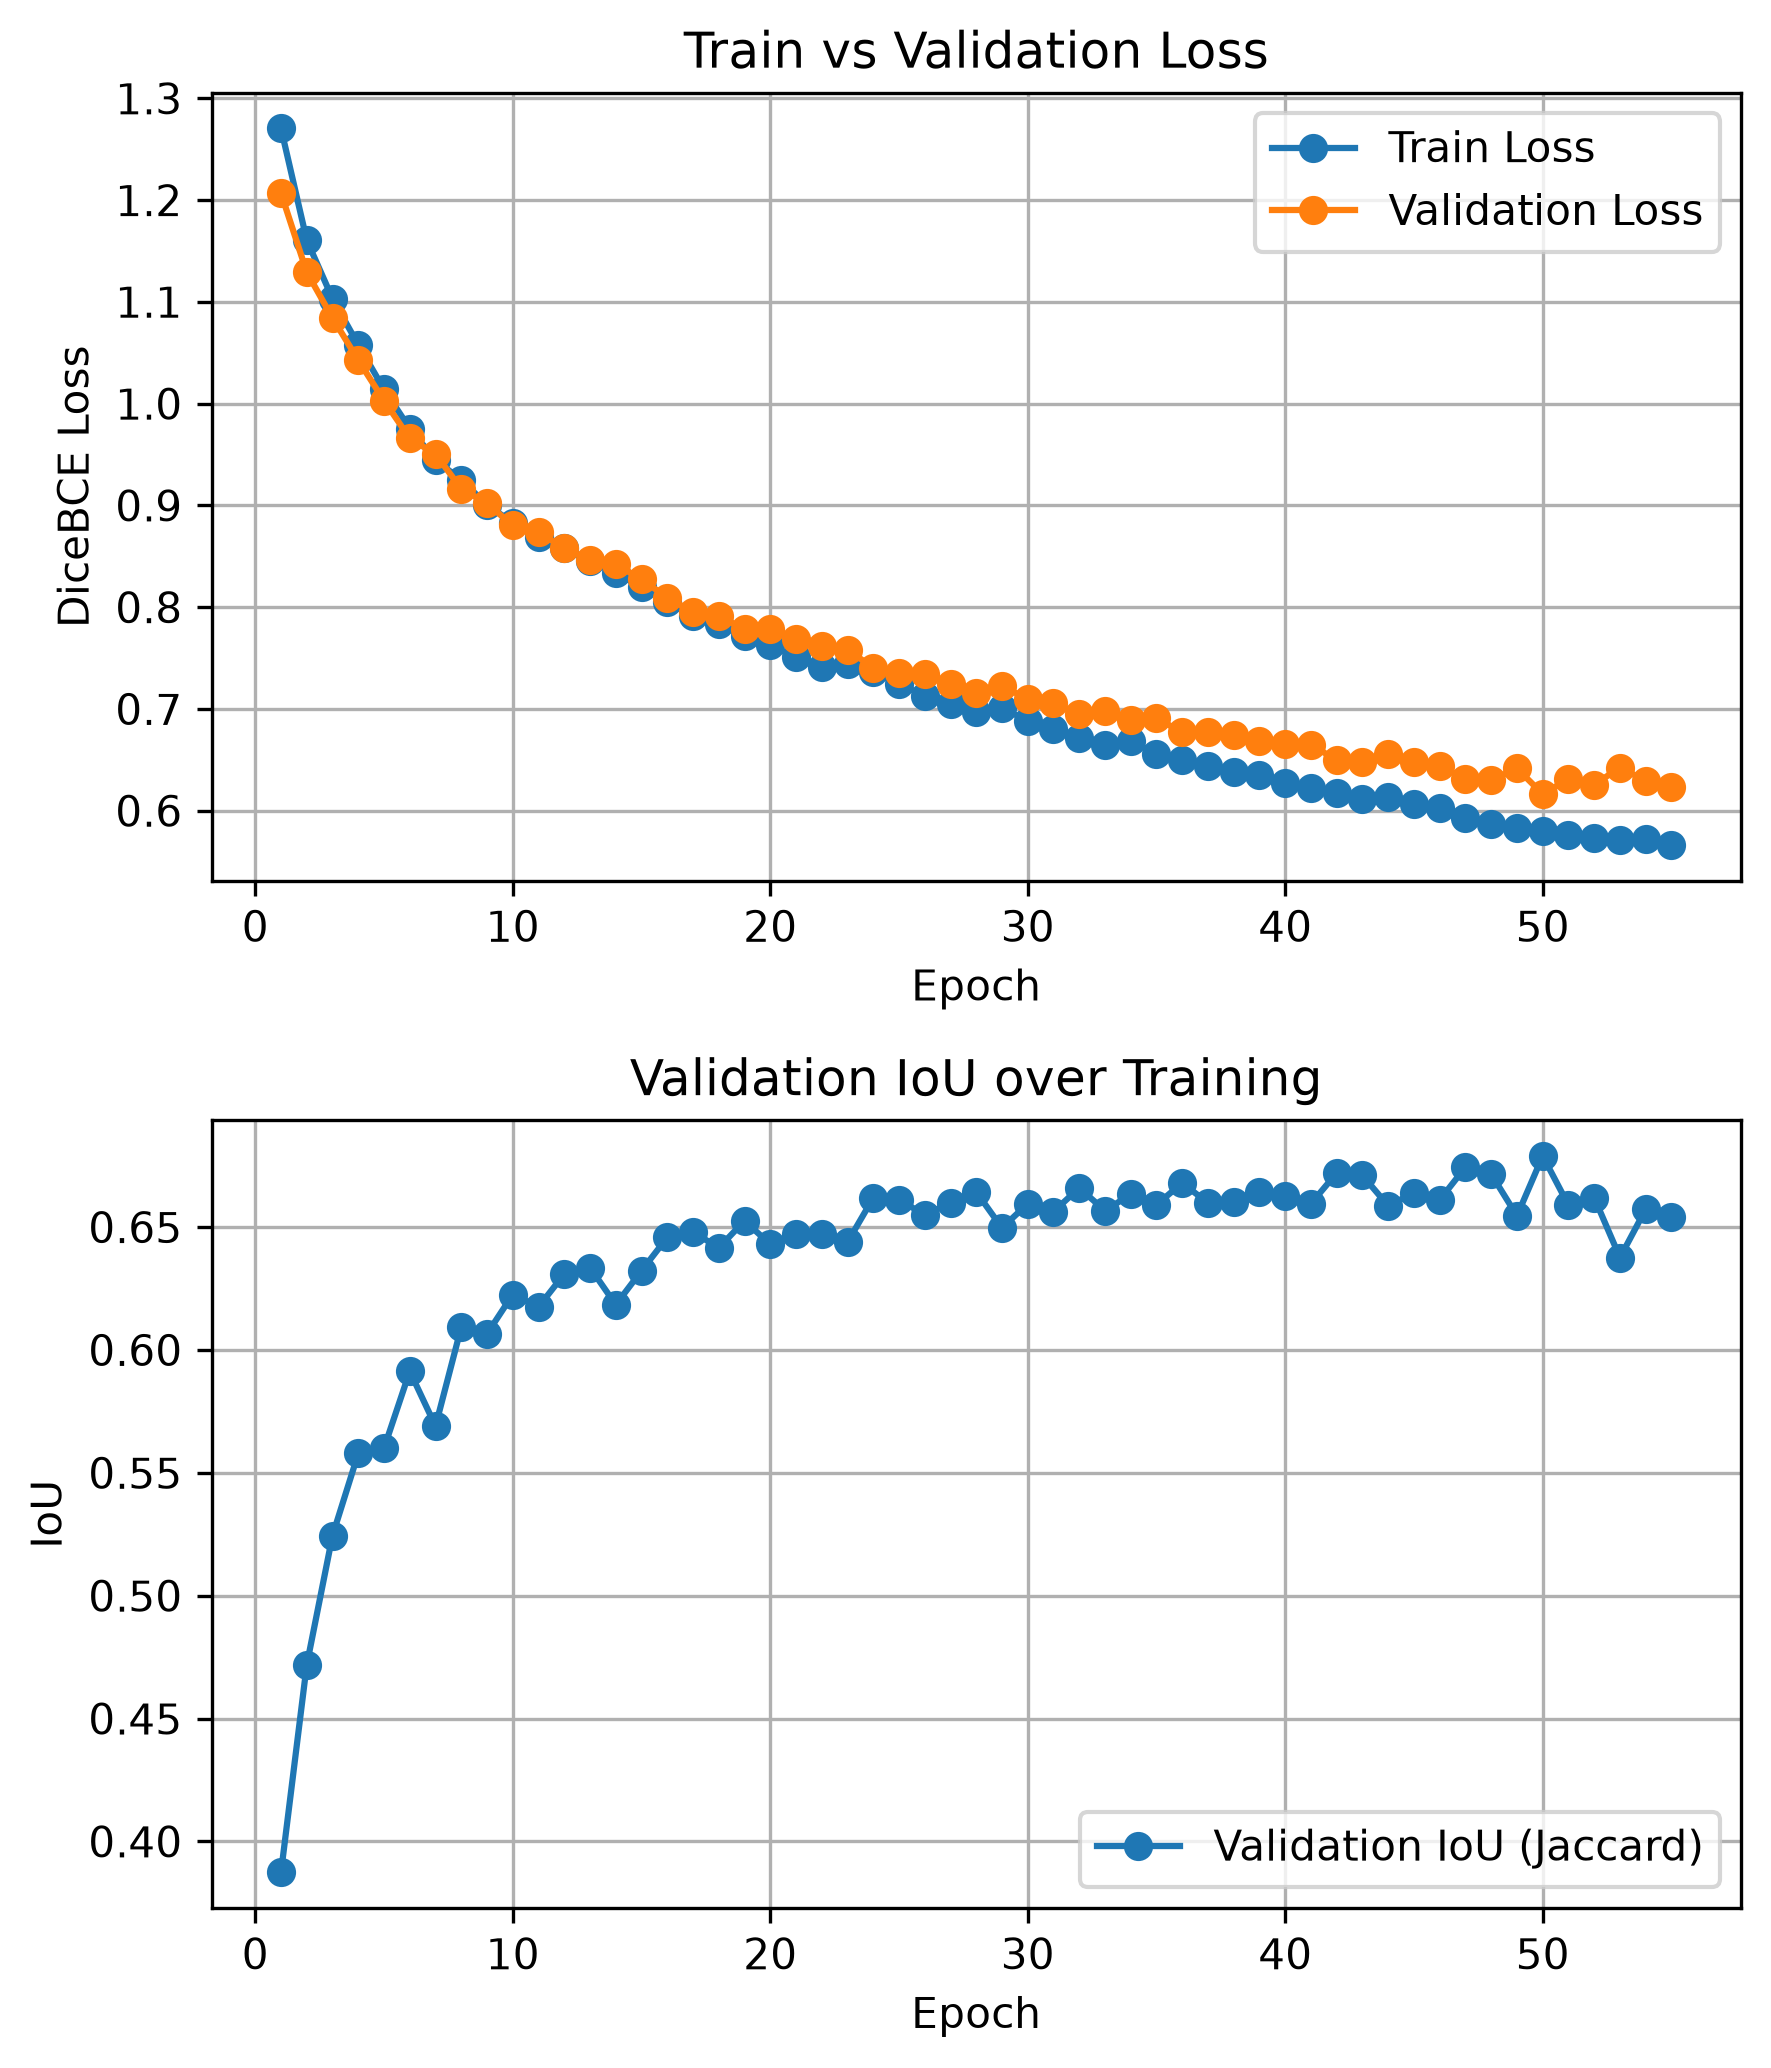
\includegraphics[width=\linewidth]{Images/unet_training_curves.png}
\caption{Training curves for Attention U-Net with DiceBCE loss.}
\label{fig:unet_curves}
\end{figure}

Table~\ref{tab:unet_perf} reports metrics computed on the full training set, as per exercise/instructor requirements.

\begin{table}[H]
\centering
\caption{Attention U-Net segmentation performance (training set).}
\label{tab:unet_perf}
\begin{tabular}{lcc}
\toprule
Metric & Value \\
\midrule
Jaccard (IoU) & 0.7167 \\
F1 Score (Dice) & 0.8348 \\
Recall (Sensitivity) & 0.8775 \\
Precision & 0.7969 \\
Accuracy & 0.9209 \\
\bottomrule
\end{tabular}
\end{table}

Figure~\ref{fig:unet_confusion} shows the pixel-level confusion matrix, computed on 4,516,320 pixels from the training set. True Positives: 906,023, False Positives: 229,576, False Negatives: 127,589, True Negatives: 3,253,132. Recall clearly exceeds precision here (87.8\% vs 79.7\%), meaning the model over-predicts membrane pixels somewhat (more false positives than false negatives) rather than missing them.

\begin{figure}[H]
\centering
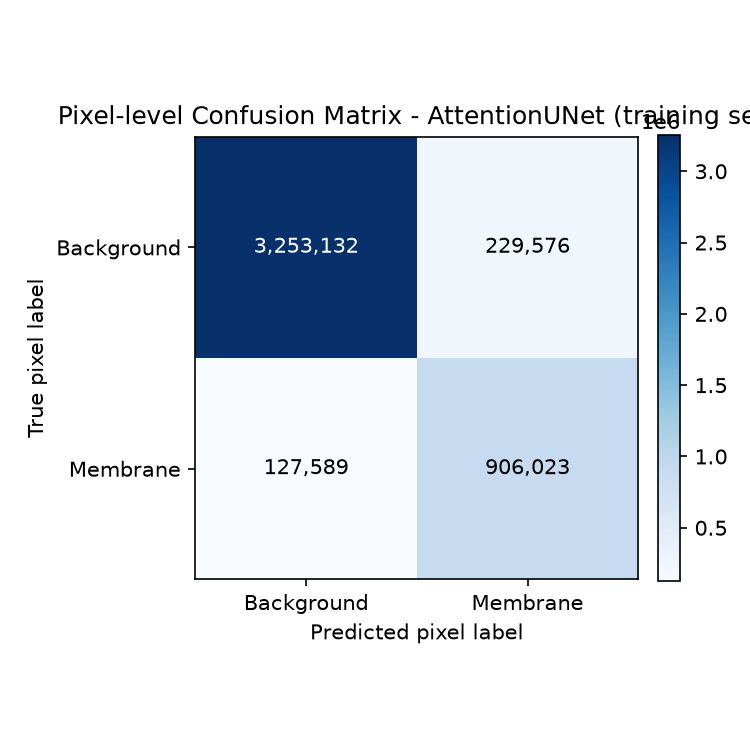
\includegraphics[width=0.8\linewidth]{Images/unet_confusion_matrix.png}
\caption{Pixel-level confusion matrix - Attention U-Net.}
\label{fig:unet_confusion}
\end{figure}

The ROC curve (Figure~\ref{fig:unet_roc}) achieved an AUC of 0.970 (computed on a 300,000-pixel subsample for tractability; the confusion matrix and Table~\ref{tab:unet_perf} use the full 4.5M pixels), demonstrating strong discrimination between membrane and background pixels, and a clear improvement over the earlier plain-UNet run's pixel-level AUC of 0.927.

\begin{figure}[H]
\centering
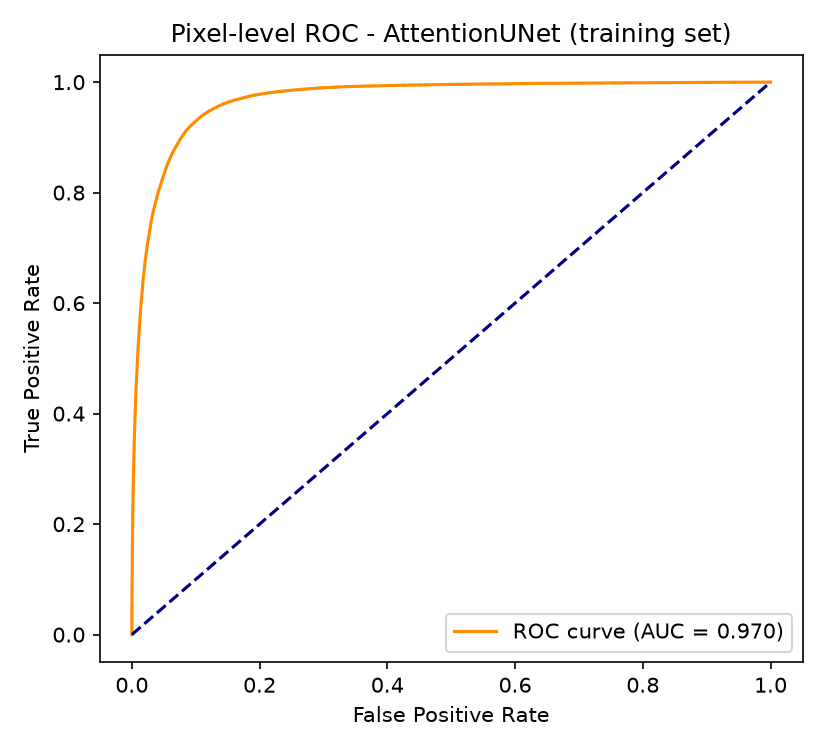
\includegraphics[width=0.8\linewidth]{Images/unet_roc.png}
\caption{Pixel-level ROC curve - Attention U-Net (AUC = 0.970).}
\label{fig:unet_roc}
\end{figure}

Table~\ref{tab:seg_comparison} compares our Attention U-Net (Dice+BCE loss) with a UNet (Dice+BCE loss) and a TransUNet (IoU+BCE loss) trained by group members on the same dataset.

\begin{table}[H]
\centering
\caption{Model comparison for membrane segmentation.}
\label{tab:seg_comparison}
\small
\setlength{\tabcolsep}{3.5pt}
\begin{tabular}{l c c c c c}
\toprule
Model / Loss & Jaccard & F1 & Recall & Prec. & Acc. \\
\midrule
Attention U-Net & 0.7167 & 0.8348 & 0.8775 & 0.7969 & 0.9209 \\
UNet (Dice+BCE) & 0.8974 & 0.9459 & 0.9464 & 0.9454 & 0.9159 \\
TransUNet (IoU+BCE) & 0.8969 & 0.9456 & 0.9373 & 0.9541 & 0.9162 \\
\bottomrule
\end{tabular}
\end{table}

The comparison reveals a significant performance gap. Both the UNet and TransUNet models substantially outperform the Attention U-Net across all metrics, achieving Jaccard scores above 0.89 compared to our model's 0.7167. This suggests that the architectural complexity and larger capacity of these models are better suited for this segmentation task, potentially allowing them to learn more robust feature representations despite the limited dataset. Our Attention U-Net's lower precision (0.7969 vs. 0.9454 and 0.9541) is consistent with the pattern seen in Figure~\ref{fig:unet_confusion}, indicating a tendency to over-predict membrane pixels. The other models achieve a significantly better balance, resulting in higher overall performance.

Note: The Jaccard and F1 scores for the UNet and TransUNet models in this table are substantially higher than those reported for our Attention U-Net in Table~\ref{tab:unet_perf}, confirming that they are more effective for this task.

Figure~\ref{fig:unet_test_predictions} shows predictions on two slices of the genuinely unlabeled test volume. The predicted segmentations capture membrane structures effectively, with fine boundary details preserved and few isolated false-positive blobs compared to the earlier plain-UNet output. The overlay visualization (Figure~\ref{fig:unet_overlay}) shows predicted membrane contours in green on the same test images.

\begin{figure}[H]
\centering
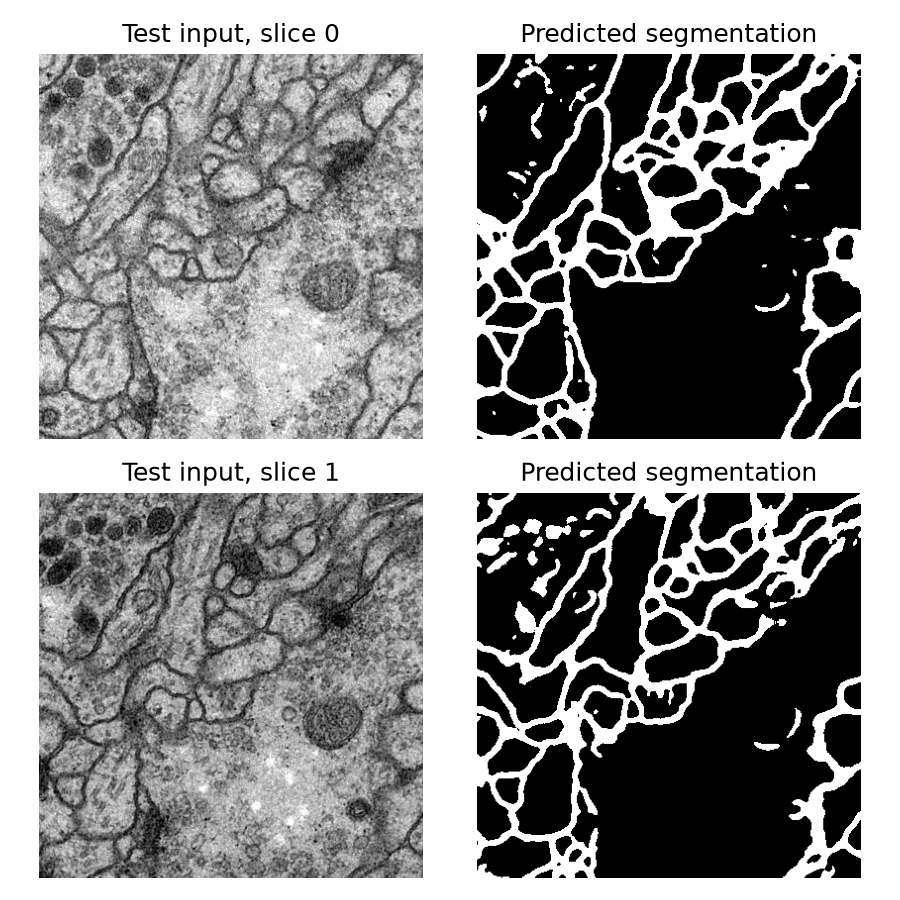
\includegraphics[width=\linewidth]{Images/unet_test_predictions.png}
\caption{Test image predictions (input and predicted segmentation), Attention U-Net.}
\label{fig:unet_test_predictions}
\end{figure}

\begin{figure}[H]
\centering
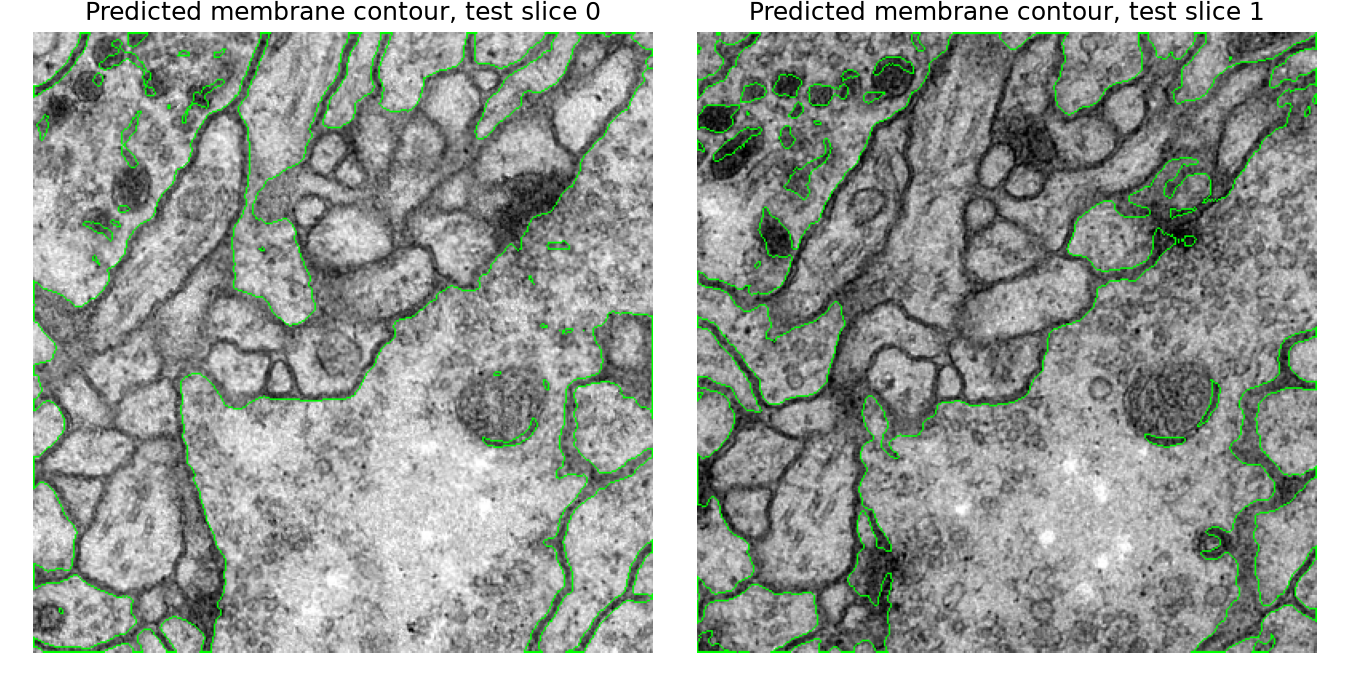
\includegraphics[width=\linewidth]{Images/unet_overlay.png}
\caption{Predicted membrane contours overlaid on test images, Attention U-Net.}
\label{fig:unet_overlay}
\end{figure}

\columnbreak
\section{Conclusion}
\textbf{Polyp Characterization:} DenseNet121 pretrained on ImageNet with transfer learning achieved strong performance (96.49\% accuracy, AUC 0.990) on the CCE polyp characterization task, with 20 of 569 test images misclassified (6 false positives, 14 false negatives) -- the PR curve's precision collapse at recall $>$0.9 reflects these hard positives. This demonstrates three key advantages: 
\begin{itemize}
	\item Transfer learning from natural images generalizes well to medical imaging.
	\item DenseNet's parameter efficiency limits overfitting on a training set of under 2000 images.
	\item Grad-CAM visualizations confirm the model focuses on clinically relevant regions.
\end{itemize}
The contrast with the scratch-trained ResNet18 (70.83\% accuracy, 93.75\% sensitivity, 25\% specificity) highlights the importance of pretraining for limited medical datasets. Sensitivity (94.19\%) trailing specificity (98.17\%) means missed neoplasia cases are the model's main error mode, which matters more clinically than false alarms.\\

\textbf{Semantic Segmentation:} Attention U-Net with DiceBCE loss produced moderate segmentation quality (Jaccard 0.717, F1/Dice 0.835, pixel-level AUC 0.970) on the ISBI 2012 neuronal membrane dataset. A comparison with other models shows that a standard UNet and a TransUNet achieve significantly higher performance (Jaccard > 0.89), suggesting that the Attention U-Net's architecture, while better than a baseline, may still be under-utilizing the available data or may be more sensitive to hyperparameter choices. Recall (87.8\%) exceeding precision (79.7\%) shows the model's main error mode is over-predicting membrane rather than missing it, the opposite pattern from under-segmentation. Training with only 24 labeled slices (30 total) remained the binding constraint; the train/validation loss gap opening after $\approx$epoch 30 indicates some overfitting despite this improvement.\\

\textbf{Limitations and Future Work:}
\begin{itemize}
	\item The CCE polyp characterization model achieved strong but imperfect performance (AUC 0.990); the 14 false negatives are the more clinically important error mode and warrant inspecting those specific cases directly. Cross-validation or evaluation on external datasets would provide more robust estimates.
	\item For segmentation, Attention U-Net used only 24 training slices; the widening train/validation loss gap after epoch 30 suggests more labeled data, stronger augmentation, or regularization could still help.
	\item For both tasks, hyperparameter optimization (learning rate, batch size, loss function weights) could yield further improvements.\\
\end{itemize}

\columnbreak

\textbf{Final Remarks:} Both tasks demonstrate the effectiveness of deep learning for medical image analysis. DenseNet121's parameter efficiency makes it ideal for small medical imaging datasets, while Attention U-Net's attention-gated skip connections provide strong localization for segmentation tasks on very small labeled sets, outperforming both a plain UNet and a dilated-backbone DeepLabV3+ baseline here. The combination of transfer learning, appropriate loss functions, and early stopping proved essential for successful training on limited medical data.

\end{multicols*}
\end{document}